%!TEX root = practicum2.tex
\begin{figure}
	\centering
	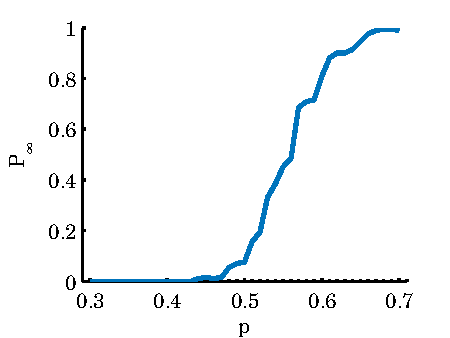
\includegraphics[width=\columnwidth]{./img/assignment_a_p_infinite_ratio_p.pdf}
	\caption{Ratio of percolating clusters, $P_\infty$, as a function of $p$. Ratios are calculated over $r_{max} = 200$ runs on a $41 \times 41$ grid.}
	\label{fig:experiment:prob:p_inf_ratio}
\end{figure}


\begin{figure*}
	\centering
	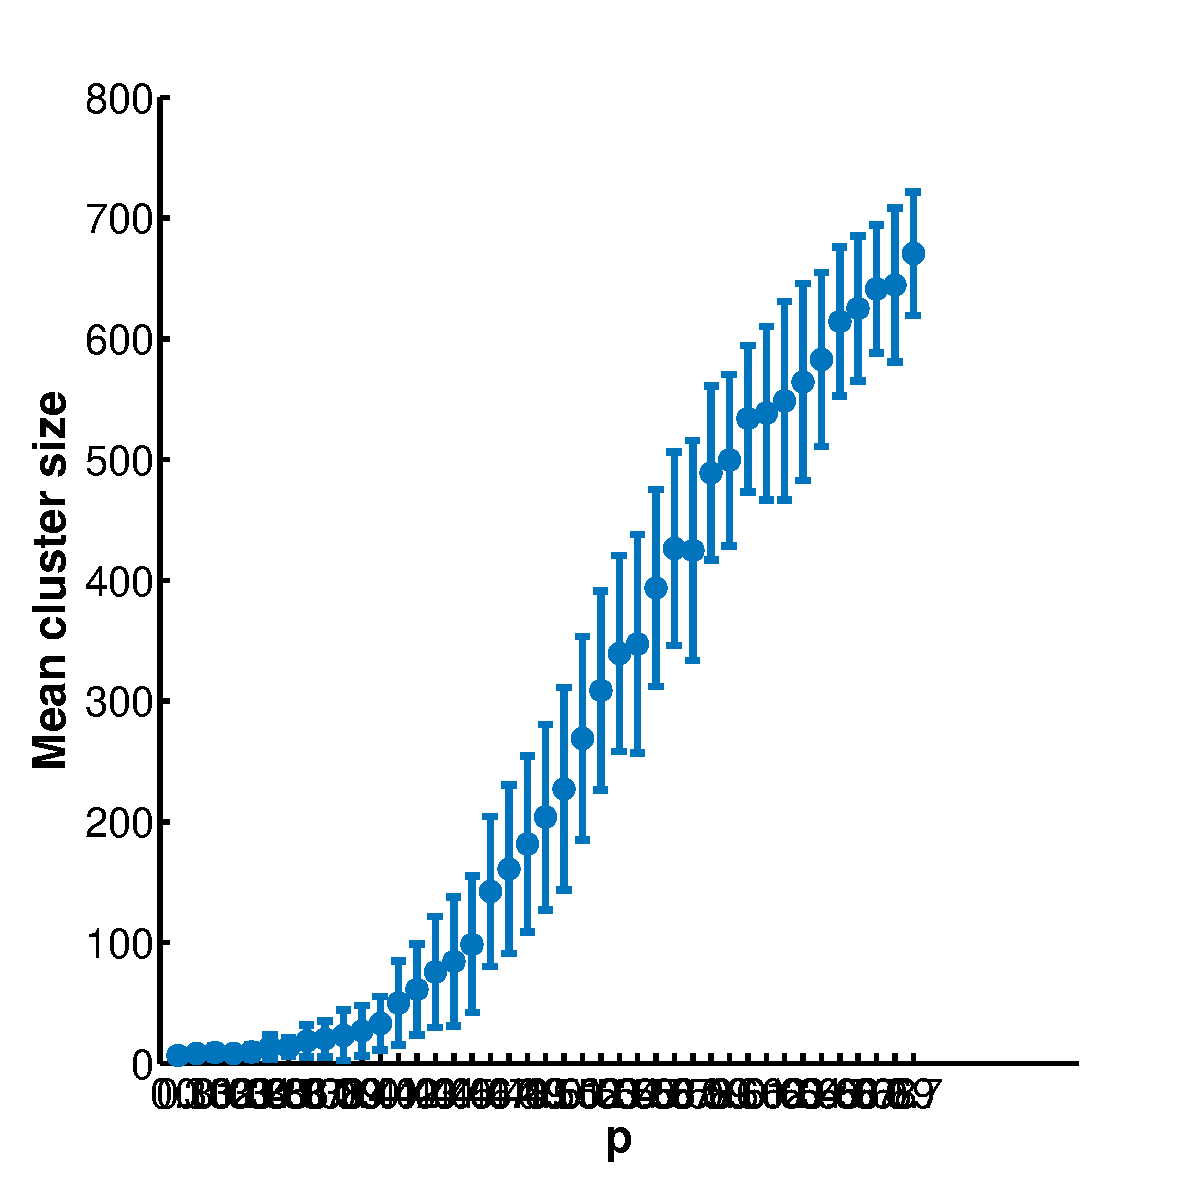
\includegraphics[width=\textwidth]{./img/assignment_a_mean_std_p.pdf}
	\caption{Mean cluster sizes, represented as points, and standard deviations, indicated by the vertical error bars, as a function of $p$, with a step size of $0.1$. The mean and standard deviation were calculated over $200$ runs on a $41 \times 41$ grid.}
	\label{fig:experiment:prob:mean_std_clusters}
\end{figure*}

% Theory
One important property of clusters is their size, and how that size depends on the parameter $p$. \textcite{kenzel1997physics} describe this relation as follows: for small values of $p$ we get a large number of small clusters. As $p$ increases we find positive correlation between $p$ and the average cluster size until $p$ reaches some threshold value $p_c$. For $p > p_c$ we get either a small finite cluster or a percolating cluster. As $p > p_c$ increases the probability of ending with a finite cluster decreases, until we always get the percolating cluster for $p =1 $. Note that although in theory this cluster should cover the full grid, this is not necessarily the case in our model, since it stops growing as soon as one border site is occupied. \\

% Ons experiment
To find an indication of the value of $p_c$ with our model we have let it generate a cluster on a $41 \times 41$ grid for $p = 0.31, 0.32, \dotsc, 0.7$. For each value of $p$ we grow $r_{max} = 200$ clusters. 

\Cref{fig:experiment:prob:mean_std_clusters} presents the mean and standard deviation of the size of the finite clusters as a function of $p$. In this figure we observe the effect of $p$ on the mean cluster size described by \citeauthor{kenzel1997physics}. Furthermore, based on these data one would estimate $p_c$ to be approximately $0.55$. 

\citeauthor{kenzel1997physics} also predicted that the number of percolating clusters relative to the number of finite clusters would grow for $p > p_c$ until $p = 1$, where the only possibility would be a percolating cluster. To observe this effect \cref{fig:experiment:prob:p_inf_ratio} shows $p_\infty$, which is the ratio of the number of percolating clusters to the number of finite clusters. This graph is based on the same data as \cref{fig:experiment:prob:mean_std_clusters}. Based on this graph we would say that $p_c \approx 0.4$. This number is lower than the value for $p_c$ based on \cref{fig:experiment:prob:mean_std_clusters}. This is probably caused by the relatively small grid sizes, which causes us to classify some clusters as percolating, that are actually finite. 

\textcite{stauffer1994introduction} has found $p_c$ to be approximately \num{0.59275} for a square lattice. As stated earlier our lower estimation of $p_c$ is quite likely caused by our small grid. 
